\documentclass[main.tex]{subfiles}
\begin{document}

\section{A Case Study and Examples: Soft Constraint Systems}\label{sec:softconstraints}
\label{subsec:inst} This section recalls
%recall the main concepts of
the key notions of the soft constraint framework, and cast it into our CLIM formalism
(following, yet generalising \cite{scc}).

\begin{definition}[Constraints]\label{def:softconstraints}
Let $V$ be a (possibly ordered)
set of variables and $D$ a finite domain of interpretation
for $V$. Then, a \emph{constraint} $(V \rightarrow D) \rightarrow
A$ is a function associating a value in $A$ to each assignment
$\eta: V\rightarrow D$ of the variables.
\end{definition}

We define ${\mathcal C}$ as the set of constraints that can be
built starting from chosen $\mathbb S$, $V$ and $D$. The application of a
constraint function $c:(V \rightarrow D) \rightarrow A$ to a variable
assignment $\eta:V\rightarrow D$ is denoted $c\eta$.  Note that even if
a constraint involves all the variables in $V$, it may depend on
the assignment of a finite subset of them, called its support. For
instance, a binary constraint $c$ with $supp(c)=\{x,y\}$ is a function
$c: (V\rightarrow D)\rightarrow A$ which depends only on the
assignment of variables $\{x,y\}\subseteq V$, meaning that two
assignments $\eta_1, \eta_2: V \rightarrow D$ differing only for the
image of variables $z \not \in \{x,y\}$ coincide (i.e., $c\eta_1 =
c\eta_2$).
%
The support corresponds to the classical notion of scope of a
constraint.  We often refer to a constraint with support $X$ as $c_X$.
Moreover, an assignment over a support $X$ of size $k$ is concisely
represented by a tuple $t$ in $D^k$ and we often write $c_X(t)$
instead of $c_X\eta$.

\smallskip
The set of constraints (with finite support) clearly forms a CLIM, where the structure
is lifted from ${\mathbb S}$.
%
Furthermore, it enjoys the cylindric properties, as shown by
the result below (due to~\cite{scc}).

\begin{proposition}[The CLIM of constraints]\label{prop:soft}
  The cylindric CLIM of constraints $\mathbb C$ is
  defined as $\langle {\mathcal C}, \leq, \otimes\rangle$ such that

  \begin{itemize}
  \item $c_1 \leq c_2$ if $c_1\eta\leq c_2\eta$ for all $\eta: V \rightarrow D$
  \item $(c_1\otimes c_2)\eta = c_1\eta\otimes c_2\eta$ for all $c_1, c_2\ \in {\mathcal C}$
  \item  $(\exists_x c) \eta = \bigwedge_{d \in D} c \eta [x:=d]$ for all $c \in {\mathcal C}, x \in V$
 \item $\delta_{x,y}\eta = \left\{
 \begin{array}{rcl} \bot & & \text{if } \eta(x) = \eta(y); \\
 \top & & \text{otherwise.}
 \end{array} \right.$ for all $x, y \in V$
  \end{itemize}
\end{proposition}

Combining two constraints by the $\otimes$ operator
means building a new constraint whose support involves at most
the variables of the original ones, and which associates with
each tuple of domain values for such variables the element
which is obtained by multiplying  those associated by the
original constraints to the appropriate sub-tuples.

Hiding means eliminating variables from the support, and indeed,
$supp(\exists_x c) \subseteq supp({c}) \setminus \{x\}$.\footnote{The operator
is called \emph{projection} in the soft framework,
and $\exists_x c$ is denoted $c\Downarrow_{V-\{x\}}$.}
%
Finally, the diagonal element $\delta_{x,y}$ has support $\{x, y\}$ for 
$x \neq y$, and $\delta_{x,x} = \bot$. Note also that these elements are not 
$\otimes$-compact.

Residuation works as expected (i.e., $(c_1\odiv c_2)\eta = c_1\eta\odiv c_2\eta$),
and top and bottom are the constant functions mapping all $\eta$ to $\top$ and $\bot$,
respectively.

\begin{definition}[Soft CSPs]
  A \emph{soft constraint satisfaction problem} is a pair $\langle C,
  Y \rangle$, where $C \subseteq {\cal C}$ is a set of constraints and
  $Y \subseteq V$ is a finite set of variables.
\end{definition}

The set $Y$ contains the variables of interest for the constraint
set $C$.

\begin{definition}[Solutions]
  The \emph{solution} of a soft CSP $P = \langle C,Y \rangle$ is
  defined as the constraint $Sol({P})=\exists_{supp(\bigotimes C) \setminus Y} \bigotimes C$.
\end{definition}

The solution of a soft CSP is obtained by combining all
constraints, and then hiding the variables that are not of interest.
%, i.e., that are not in $Y$.
%
In this way we get the constraint with support (not greater than) $Y$
``induced'' by the entire CSP.

\smallskip
A tightly related notion, one which is quite important in
combinatorial optimisation problems, is the best level of
consistency~\cite{jacm}.
%Note that when all the
%variables are of interest we do not need to perform any projection.

\begin{definition}
  The \emph{Best level of consistency} of a soft CSP problem $P =
  \langle C,Y \rangle$ is defined as the constraint $blevel(P) =
  \exists_Y Sol({P})$.
  % A problem $P$ is $\alpha$-consistent if $blevel(P) = \alpha$; $P$
  % is instead simply ``consistent'' iff there exists $\alpha >_S \0$
  % such that $P$ is $\alpha$-consistent~\cite{bistabook}. $P$ is
  % inconsistent if it is not consistent.
\end{definition}


%Consider the  set $\C$ and the partial order
%$\sqsubseteq$. The entailment relation $\ent \, \subseteq \C
%\times \C$ is defined such that for each  $c_1, c_2 \in
%\C$, we have $c_1 \ent c_2$ if and only if $c_1 \sqsubseteq c_2$ and $supp(c_2) \subseteq supp(c_1)$: for instance, a %constraint supported by $x$ and $y$ cannot entail any constraint defined over variable $z$.
%\marginpar{Questo paragrafo era nella sezione originale. Non mi torna la condizione sul supporto con $\top$ e $\bot$. %Check Prop. 1}

\begin{figure}
\centering
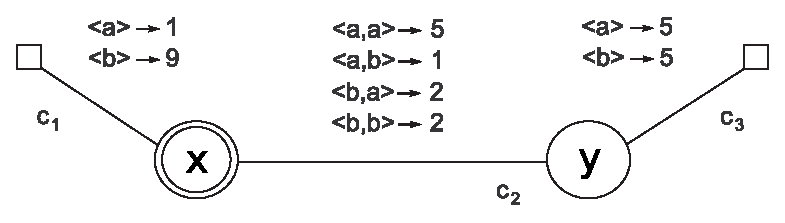
\includegraphics[scale=0.57]{wexample.eps} %0.43
\caption{A soft CSP based on a Weighted CLIM.}
\label{figure:wexample}
\end{figure}

\begin{example}
\label{ex1}
Figure~\ref{figure:wexample}
shows a weighted CSP as a graph with values from
the CLIM $\langle \mathbb{R}^{+}, \leq, +\rangle$ (the \emph{Weighted} semiring, in the soft CSP jargon):
the non-negative reals plus $\infty$ with the standard order and addition as monoidal operator.
%
Variables and constraints are represented respectively by nodes
and by undirected arcs (unary for $c_1$ and $c_3$, and binary for
$c_2$), and values are written to the right of each
tuple. The variables of interest are
represented with a double circle (i.e. variable $x$). We
assume that the domain of the variables contains only elements $a$
and $b$. The solution of the weighted CSP of
Figure~\ref{figure:wexample} associates an element to every
domain value of variable $x$. Such an element is obtained by first
combining all the constraints together. For instance, for the
tuple $\langle a, a\rangle$ (that is, $x = y = a$), we have to
compute the sum of $1$ (the value assigned to $x = a$ in
constraint $c_1$), $5$ (the value assigned to $\langle x
= a, y = a \rangle$ in $c_2$) and $5$ (the value assigned to $y =
a$ in $c_3$). Hence, the resulting value for this tuple is $11$.
We can repeat the same procedure for tuple $\langle a, b\rangle \rightarrow
7$, $\langle b, a\rangle \rightarrow 16$ and $\langle b, b\rangle
\rightarrow 16$. The variable $y$ is then hidden in the resulting tuples,
obtaining the solution $\langle a \rangle \rightarrow
7$ and $\langle b \rangle \rightarrow 16$. The \emph{blevel} for
the example in Figure~\ref{figure:wexample} is $7$ (related to the
solution $x = a$, $y = b$).
\end{example}

\section{Examples of Computation}\label{sec:examples}
In the following we provide some examples of agent computations to clarify the  semantics in Table~\ref{fig:operational} and Table~\ref{fig:operational2}: we curb to the unlabelled versions without loss of generality, dropping the trailing $\stopp$ whenever in parallel with another agent. 
%
We adopt the CLIM $\langle \mathbb{R}^{+}, \leq, +\rangle$, which considers  non-negative reals plus $\infty$ with the standard order, and addition as the monoidal operator. We also consider two constraints $c_1 = x+1$ ($\mathit{sv}(c_1)= \{x\}$) and $c_2= y+2$ ($\mathit{sv}(c_2)= \{y\}$). 

\begin{example}[Tell, ask, and parallel operators]
	We start with the querying agent $\ask(c_1)$, executed in a store $c_1 \otimes c_2$: since $c_1 \leq c_1 \otimes c_2$, $\mathit{sv}(c_1 \otimes c_2) = \{x,y\}$, and $\mathit{sv}(c_1) = \{x\}$, using Table~\ref{fig:operational} we get
	$\langle \ask(c_1) \rightarrow \stopp, c_1 \otimes c_2 \rangle \mapsto_{\{x,y\}} \langle \stopp, c_1 \otimes c_2 \rangle$.
	
	Next example uses two agents in parallel each adding a different constraint.
    As stated in the precondition of rules {\bf R1}-{\bf R2} in Table~\ref{fig:operational2}, the free variables of the suspended branch (i.e., $\mathit{fv(B)}$) have to be in 
    the subscript $\Delta$ as well, since $\Delta$ collects all the variables that are going to be used in all the branches. As an example, since $\mathit{fv}(\tell(c_2))= \mathit{sv}(c_2) = {y}$, then
$\langle \tell(c_1) \parallel \tell(c_2), \bot \rangle \mapsto_{\{x,y\}} \langle \tell(c_2), c_1 \rangle \mapsto_{\{x,y\}} \langle \stopp, c_1 \otimes c_2\rangle$.
	\normalsize
\end{example}


\begin{example}[Procedure call and hiding]
	
	Rule {\bf A3} in Table~\ref{fig:operational} just requires the actual parameter $y$ to be in the subscript
	$\Delta$ (together with the support variables of the global store, in this case $\mathit{sv}(c_1)= \{x\}$); then, it applies a straight renaming of the formal parameter with the actual one. An example is given below, where we suppose to have  $p(x) = \exists_x \tell(c_1)$ among the procedures declared in   $\mathcal{P}$, so that 
	$\langle p(y), c_1 \rangle \mapsto_{\{x,y\}} \langle \exists_y \tell(c_1[^y/_x]), c_1\rangle \dots$
	
	Note that, by substituting $x$ with $y$ in $c_1$ (i.e., $c_1[^y/_x]$), the value becomes $y + 1$ (see Definition~\ref{def:sub}, and Proposition~\ref{prop:soft} for the operator instantiations): in words, the value of $x$ in $c_1$ is passed to $y$ with a diagonal constraint ($\delta_{x,y} \otimes c_1$), and then the influence of $x$ is removed from $c_1$ through the cylindric operator: $\exists_x (\delta_{x,y} \otimes c_1)$. The  next step concerns the hiding operator: rule {\bf A4} in Table~\ref{fig:operational} requires as precondition a fresh name $w$ ($w \not\in \{x,y\}$) that is used to rename the hidden variable $y$. In this case, $y$ is renamed with $w$ in $c_1$ (thus, $d = w+1$, see Proposition~\ref{prop:soft}), and $w$ is then added to the subscript $\Delta$ because of the tell action
	$\dots \langle \exists_y \tell(c_1[^y/_x]), c_1\rangle \mapsto_{\{x,y\}} \langle \tell((c_1[^y/_x])[^w/_y]), c_1 \rangle \mapsto_{\{x,y,w\}} \langle \stopp, c_1 \otimes d \rangle$.
	
	Therefore, the final store is $c_1 \otimes d= x + w + 2$; notice that $y$ has been recorded as used, but it is no longer present in the global store.\footnote{Note 
	$\mathit{sv}(c \otimes d) \subseteq \mathit{sv(c)} \cup \mathit{sv(d)}$, differently from what stated in \cite{scc}, where $=$ is assumed.}
\end{example}

Fairness represents a large class of infinitary properties, usually viewed as a subclass of liveness properties (i.e., \emph{``something good happens''}). Such properties restrict the set of potential computations of a system by disallowing those infinite computations that indefinitely delay some system component~\cite{fairness}. 
%One characteristic feature of these properties is that one has to consider also infinite computations besides finites ones. 
Fairness is known to affect liveness properties: the correctness of a program with respect to some property cannot be proved unless its infinite computations are restricted to just the fair ones.  Unfortunately, transition rules defined in classical SCCP~\cite{scc} do not consider infinite computations (crisp constraint-languages often treat them as failures~\cite{fairness}), something that we solve in this work instead. The next example illustrates how fair computations can be  captured by the use of $\Delta$ with the semantics using a global store (Section~\ref{sec:detSCCP}). 

\begin{example}[Fair computations] In the following we consider an interaction $A \parallel B$ between a sequencer agent $B$ that marks the rhythm of agent $A$, which in turn has the task to progressively consume an infinite resource by adding $c_r$ each time. Constraints are indexed with their support variable, i.e., $c_x$, $c_y$, and $c_r$. $A$ waits for $B$ to grant permission to add $c_r$ via a signal on $c_x$: when $c_x$ is in the store, $A$ adds $c_r$. When $A$ finishes, it informs $B$ by telling $c_y$, and $B$, hanging on the corresponding $\ask(c_y)$, is then unblocked. Finally, $B$ launches the same parallel computation after changing the signalling variables $x$ and $y$ by renaming them (in the same way for both $A$ and $B$). Two procedures $p_1(x,y)$ and $p_2(x,y)$ replicate the behaviour of the initial agents, so that they can be invoked infinite times.
 %
 \[A = p_1(x,y): \ask(c_x) \rrarrow \tell(c_y \otimes c_r)\]
 \[B = p_2(x,y): \tell(c_x) \parallel (\ask(c_y) \rrarrow \exists_{\{x,y\}} (p_1(x,y) \parallel p_2(x,y)))\]
 %
 Looking now at the reduction semantics provided in Table~\ref{fig:operational}, the first observables are described from Eq.~\ref{obs:1} to 
 Eq.~\ref{obs:last}
 %
 \begin{equation}\label{obs:1}
 \langle A \parallel B, \bot \rangle \rrarrow_{\{r,x,y\}} \langle A \parallel \ask(c_y) \rrarrow \exists_{\{r,x,y\}} (p_1(x,y) \parallel p_2(x,y)), c_x \rangle
 \end{equation}
 %
 \begin{equation}
 \begin{split}
 \langle \tell(c_y \otimes c_r) \parallel \ask(c_y) \rrarrow \exists_{\{r,x,y\}} (p_1(x,y) \parallel p_2(x,y)), c_x\rangle \rrarrow_{\{r,x,y\}}\\ \langle \tell(c_y \otimes c_r) \parallel 
  \ask(c_y) \rrarrow \exists_{\{r,x,y\}} (p_1(x,y) \parallel p_2(x,y)), c_x\rangle
 \end{split}
 \end{equation}
 %
  \begin{equation}
  \begin{split}
  \langle \tell(c_y \otimes c_r) \parallel \ask(c_y) \rrarrow \exists_{\{r,x,y\}} (p_1(x,y) \parallel p_2(x,y)), c_x \rangle \rrarrow_{\{r,x,y\}}\\ \langle \ask(c_y) \rrarrow \exists_{\{r,x,y\}} (p_1(x,y) \parallel p_2(x,y)), c_x \otimes c_y \otimes c_r\rangle
  \end{split}
  \end{equation}
  %
    \begin{equation}
    \begin{split}
    \langle \ask(c_y) \rrarrow \exists_{\{r,x,y\}} (p_1(x,y) \parallel p_2(x,y)), c_x\rangle \rrarrow_{\{r,x,y\}}\\ \langle \exists_{\{r,x,y\}} (p_1(x,y) \parallel p_2(x,y)), c_x \otimes c_y \otimes c_r\rangle
    \end{split}
    \end{equation}
  %
  Then, if we rename $x$ with $v$ and $y$ with $w$ we have
  %
     \begin{equation}
      \begin{split}
      \langle \exists_{\{r,x,y\}} (p_1(x,y) \parallel p_2(x,y)), c_x \otimes c_r \otimes c_y \otimes c_r\rangle  \rrarrow_{\{r,x,y\}}\\ \langle p_1(x,y)[^v/_x][^w/_y] \parallel p_2(x,y)[^v/_x][^w/_y], c_x \otimes c_y \otimes c_r\rangle
      \end{split}
      \end{equation}
     %
      where $p_1(x,y)[^v/_x][^w/_y] = p_1(v,w)$ and $p_2(x,y)[^v/_x][^w/_y] = p_2(v,w)$. Then, if $p_1(v,w)$ is invoked first
      %
      \begin{equation}
      \begin{split}
      \langle p_1(v,w) \parallel p_2(v,w), c_x \otimes c_y \otimes c_r\rangle \rrarrow_{\{r,v,w,x,y\}}\\ \langle  \ask(c_v) \rrarrow \tell(c_w \otimes c_r) \parallel p_2(v,w), c_x\otimes c_y \otimes c_r\rangle 
      \end{split}
      \end{equation}
      %
      where $c_v = c_x[^v/_x]$ and $c_w = c_y \otimes c_r[^w/_y]$. finally, also $p_2(v,w)$ is invoked
      %
      \begin{equation}\label{obs:last}
      \begin{split}
      \langle \ask(c_v) \rrarrow \tell(c_w \otimes c_r) \parallel p_2(v,w), c_x \otimes c_y \otimes c_r\rangle \rrarrow_{\{r,v,w,x,y\}} \\ \langle \ask(c_v) \rrarrow \tell(c_w \otimes c_r) \parallel \tell(c_v) \parallel \\ \ask(c_w) \rrarrow \exists_{\{v,w\}} (p_1(v,w) \parallel p_2(v,w)), c_x \otimes c_y \otimes c_r\rangle
      \end{split}
      \end{equation}
      %
Then the computation continues as in Eq.~\ref{obs:1}, and so on. Note that the presented computation is fair because it satisfies Definition~\ref{def:fair}.
\end{example}


\end{document}